% Options for packages loaded elsewhere
\PassOptionsToPackage{unicode}{hyperref}
\PassOptionsToPackage{hyphens}{url}
\PassOptionsToPackage{dvipsnames,svgnames,x11names}{xcolor}
%
\documentclass[
  letterpaper,
  DIV=11,
  numbers=noendperiod]{scrartcl}

\usepackage{amsmath,amssymb}
\usepackage{iftex}
\ifPDFTeX
  \usepackage[T1]{fontenc}
  \usepackage[utf8]{inputenc}
  \usepackage{textcomp} % provide euro and other symbols
\else % if luatex or xetex
  \usepackage{unicode-math}
  \defaultfontfeatures{Scale=MatchLowercase}
  \defaultfontfeatures[\rmfamily]{Ligatures=TeX,Scale=1}
\fi
\usepackage{lmodern}
\ifPDFTeX\else  
    % xetex/luatex font selection
\fi
% Use upquote if available, for straight quotes in verbatim environments
\IfFileExists{upquote.sty}{\usepackage{upquote}}{}
\IfFileExists{microtype.sty}{% use microtype if available
  \usepackage[]{microtype}
  \UseMicrotypeSet[protrusion]{basicmath} % disable protrusion for tt fonts
}{}
\makeatletter
\@ifundefined{KOMAClassName}{% if non-KOMA class
  \IfFileExists{parskip.sty}{%
    \usepackage{parskip}
  }{% else
    \setlength{\parindent}{0pt}
    \setlength{\parskip}{6pt plus 2pt minus 1pt}}
}{% if KOMA class
  \KOMAoptions{parskip=half}}
\makeatother
\usepackage{xcolor}
\setlength{\emergencystretch}{3em} % prevent overfull lines
\setcounter{secnumdepth}{-\maxdimen} % remove section numbering
% Make \paragraph and \subparagraph free-standing
\makeatletter
\ifx\paragraph\undefined\else
  \let\oldparagraph\paragraph
  \renewcommand{\paragraph}{
    \@ifstar
      \xxxParagraphStar
      \xxxParagraphNoStar
  }
  \newcommand{\xxxParagraphStar}[1]{\oldparagraph*{#1}\mbox{}}
  \newcommand{\xxxParagraphNoStar}[1]{\oldparagraph{#1}\mbox{}}
\fi
\ifx\subparagraph\undefined\else
  \let\oldsubparagraph\subparagraph
  \renewcommand{\subparagraph}{
    \@ifstar
      \xxxSubParagraphStar
      \xxxSubParagraphNoStar
  }
  \newcommand{\xxxSubParagraphStar}[1]{\oldsubparagraph*{#1}\mbox{}}
  \newcommand{\xxxSubParagraphNoStar}[1]{\oldsubparagraph{#1}\mbox{}}
\fi
\makeatother

\usepackage{color}
\usepackage{fancyvrb}
\newcommand{\VerbBar}{|}
\newcommand{\VERB}{\Verb[commandchars=\\\{\}]}
\DefineVerbatimEnvironment{Highlighting}{Verbatim}{commandchars=\\\{\}}
% Add ',fontsize=\small' for more characters per line
\usepackage{framed}
\definecolor{shadecolor}{RGB}{241,243,245}
\newenvironment{Shaded}{\begin{snugshade}}{\end{snugshade}}
\newcommand{\AlertTok}[1]{\textcolor[rgb]{0.68,0.00,0.00}{#1}}
\newcommand{\AnnotationTok}[1]{\textcolor[rgb]{0.37,0.37,0.37}{#1}}
\newcommand{\AttributeTok}[1]{\textcolor[rgb]{0.40,0.45,0.13}{#1}}
\newcommand{\BaseNTok}[1]{\textcolor[rgb]{0.68,0.00,0.00}{#1}}
\newcommand{\BuiltInTok}[1]{\textcolor[rgb]{0.00,0.23,0.31}{#1}}
\newcommand{\CharTok}[1]{\textcolor[rgb]{0.13,0.47,0.30}{#1}}
\newcommand{\CommentTok}[1]{\textcolor[rgb]{0.37,0.37,0.37}{#1}}
\newcommand{\CommentVarTok}[1]{\textcolor[rgb]{0.37,0.37,0.37}{\textit{#1}}}
\newcommand{\ConstantTok}[1]{\textcolor[rgb]{0.56,0.35,0.01}{#1}}
\newcommand{\ControlFlowTok}[1]{\textcolor[rgb]{0.00,0.23,0.31}{\textbf{#1}}}
\newcommand{\DataTypeTok}[1]{\textcolor[rgb]{0.68,0.00,0.00}{#1}}
\newcommand{\DecValTok}[1]{\textcolor[rgb]{0.68,0.00,0.00}{#1}}
\newcommand{\DocumentationTok}[1]{\textcolor[rgb]{0.37,0.37,0.37}{\textit{#1}}}
\newcommand{\ErrorTok}[1]{\textcolor[rgb]{0.68,0.00,0.00}{#1}}
\newcommand{\ExtensionTok}[1]{\textcolor[rgb]{0.00,0.23,0.31}{#1}}
\newcommand{\FloatTok}[1]{\textcolor[rgb]{0.68,0.00,0.00}{#1}}
\newcommand{\FunctionTok}[1]{\textcolor[rgb]{0.28,0.35,0.67}{#1}}
\newcommand{\ImportTok}[1]{\textcolor[rgb]{0.00,0.46,0.62}{#1}}
\newcommand{\InformationTok}[1]{\textcolor[rgb]{0.37,0.37,0.37}{#1}}
\newcommand{\KeywordTok}[1]{\textcolor[rgb]{0.00,0.23,0.31}{\textbf{#1}}}
\newcommand{\NormalTok}[1]{\textcolor[rgb]{0.00,0.23,0.31}{#1}}
\newcommand{\OperatorTok}[1]{\textcolor[rgb]{0.37,0.37,0.37}{#1}}
\newcommand{\OtherTok}[1]{\textcolor[rgb]{0.00,0.23,0.31}{#1}}
\newcommand{\PreprocessorTok}[1]{\textcolor[rgb]{0.68,0.00,0.00}{#1}}
\newcommand{\RegionMarkerTok}[1]{\textcolor[rgb]{0.00,0.23,0.31}{#1}}
\newcommand{\SpecialCharTok}[1]{\textcolor[rgb]{0.37,0.37,0.37}{#1}}
\newcommand{\SpecialStringTok}[1]{\textcolor[rgb]{0.13,0.47,0.30}{#1}}
\newcommand{\StringTok}[1]{\textcolor[rgb]{0.13,0.47,0.30}{#1}}
\newcommand{\VariableTok}[1]{\textcolor[rgb]{0.07,0.07,0.07}{#1}}
\newcommand{\VerbatimStringTok}[1]{\textcolor[rgb]{0.13,0.47,0.30}{#1}}
\newcommand{\WarningTok}[1]{\textcolor[rgb]{0.37,0.37,0.37}{\textit{#1}}}

\providecommand{\tightlist}{%
  \setlength{\itemsep}{0pt}\setlength{\parskip}{0pt}}\usepackage{longtable,booktabs,array}
\usepackage{calc} % for calculating minipage widths
% Correct order of tables after \paragraph or \subparagraph
\usepackage{etoolbox}
\makeatletter
\patchcmd\longtable{\par}{\if@noskipsec\mbox{}\fi\par}{}{}
\makeatother
% Allow footnotes in longtable head/foot
\IfFileExists{footnotehyper.sty}{\usepackage{footnotehyper}}{\usepackage{footnote}}
\makesavenoteenv{longtable}
\usepackage{graphicx}
\makeatletter
\def\maxwidth{\ifdim\Gin@nat@width>\linewidth\linewidth\else\Gin@nat@width\fi}
\def\maxheight{\ifdim\Gin@nat@height>\textheight\textheight\else\Gin@nat@height\fi}
\makeatother
% Scale images if necessary, so that they will not overflow the page
% margins by default, and it is still possible to overwrite the defaults
% using explicit options in \includegraphics[width, height, ...]{}
\setkeys{Gin}{width=\maxwidth,height=\maxheight,keepaspectratio}
% Set default figure placement to htbp
\makeatletter
\def\fps@figure{htbp}
\makeatother

\KOMAoption{captions}{tableheading}
\makeatletter
\@ifpackageloaded{caption}{}{\usepackage{caption}}
\AtBeginDocument{%
\ifdefined\contentsname
  \renewcommand*\contentsname{Table of contents}
\else
  \newcommand\contentsname{Table of contents}
\fi
\ifdefined\listfigurename
  \renewcommand*\listfigurename{List of Figures}
\else
  \newcommand\listfigurename{List of Figures}
\fi
\ifdefined\listtablename
  \renewcommand*\listtablename{List of Tables}
\else
  \newcommand\listtablename{List of Tables}
\fi
\ifdefined\figurename
  \renewcommand*\figurename{Figure}
\else
  \newcommand\figurename{Figure}
\fi
\ifdefined\tablename
  \renewcommand*\tablename{Table}
\else
  \newcommand\tablename{Table}
\fi
}
\@ifpackageloaded{float}{}{\usepackage{float}}
\floatstyle{ruled}
\@ifundefined{c@chapter}{\newfloat{codelisting}{h}{lop}}{\newfloat{codelisting}{h}{lop}[chapter]}
\floatname{codelisting}{Listing}
\newcommand*\listoflistings{\listof{codelisting}{List of Listings}}
\makeatother
\makeatletter
\makeatother
\makeatletter
\@ifpackageloaded{caption}{}{\usepackage{caption}}
\@ifpackageloaded{subcaption}{}{\usepackage{subcaption}}
\makeatother

\ifLuaTeX
  \usepackage{selnolig}  % disable illegal ligatures
\fi
\usepackage{bookmark}

\IfFileExists{xurl.sty}{\usepackage{xurl}}{} % add URL line breaks if available
\urlstyle{same} % disable monospaced font for URLs
\hypersetup{
  pdftitle={Education},
  pdfauthor={Gilchrist Ouedraogo},
  colorlinks=true,
  linkcolor={blue},
  filecolor={Maroon},
  citecolor={Blue},
  urlcolor={Blue},
  pdfcreator={LaTeX via pandoc}}


\title{Education}
\author{Gilchrist Ouedraogo}
\date{}

\begin{document}
\maketitle


\section{Chargement des librairies}\label{chargement-des-librairies}

\begin{Shaded}
\begin{Highlighting}[]
\FunctionTok{library}\NormalTok{(tidyverse)}
\end{Highlighting}
\end{Shaded}

\begin{verbatim}
Warning: le package 'tidyverse' a été compilé avec la version R 4.3.3
\end{verbatim}

\begin{verbatim}
Warning: le package 'ggplot2' a été compilé avec la version R 4.3.3
\end{verbatim}

\begin{verbatim}
Warning: le package 'dplyr' a été compilé avec la version R 4.3.3
\end{verbatim}

\begin{verbatim}
-- Attaching core tidyverse packages ------------------------ tidyverse 2.0.0 --
v dplyr     1.1.4     v readr     2.1.4
v forcats   1.0.0     v stringr   1.5.1
v ggplot2   3.5.1     v tibble    3.2.1
v lubridate 1.9.3     v tidyr     1.3.0
v purrr     1.0.2     
-- Conflicts ------------------------------------------ tidyverse_conflicts() --
x dplyr::filter() masks stats::filter()
x dplyr::lag()    masks stats::lag()
i Use the conflicted package (<http://conflicted.r-lib.org/>) to force all conflicts to become errors
\end{verbatim}

\begin{Shaded}
\begin{Highlighting}[]
\FunctionTok{library}\NormalTok{(questionr)}
\end{Highlighting}
\end{Shaded}

\begin{verbatim}
Warning: le package 'questionr' a été compilé avec la version R 4.3.3
\end{verbatim}

\section{Chargement de la data}\label{chargement-de-la-data}

\begin{Shaded}
\begin{Highlighting}[]
\NormalTok{df }\OtherTok{\textless{}{-}} \FunctionTok{read\_csv2}\NormalTok{(}\StringTok{"data/student{-}mat.csv"}\NormalTok{)}
\end{Highlighting}
\end{Shaded}

\begin{verbatim}
i Using "','" as decimal and "'.'" as grouping mark. Use `read_delim()` for more control.
\end{verbatim}

\begin{verbatim}
Rows: 395 Columns: 33
-- Column specification --------------------------------------------------------
Delimiter: ";"
chr (17): school, sex, address, famsize, Pstatus, Mjob, Fjob, reason, guardi...
dbl (16): age, Medu, Fedu, traveltime, studytime, failures, famrel, freetime...

i Use `spec()` to retrieve the full column specification for this data.
i Specify the column types or set `show_col_types = FALSE` to quiet this message.
\end{verbatim}

\section{Les élèves qui étudient plus obtiennent-ils de meilleures notes
?}\label{les-uxe9luxe8ves-qui-uxe9tudient-plus-obtiennent-ils-de-meilleures-notes}

Analyse de la relation entre la variable studytime et les notes (G1, G2,
G3). Une régression linéaire pourrait montrer s'il existe une
corrélation positive.

\begin{Shaded}
\begin{Highlighting}[]
\NormalTok{data }\OtherTok{\textless{}{-}}\NormalTok{ df }\SpecialCharTok{\%\textgreater{}\%} \FunctionTok{select}\NormalTok{(sex ,age ,Medu, Fedu, Mjob, Fjob,studytime, famsup,nursery, higher, internet,famrel, absences, G1, G2, G3 )}

\NormalTok{internet }\OtherTok{\textless{}{-}}\NormalTok{ data }\SpecialCharTok{\%\textgreater{}\%} \FunctionTok{count}\NormalTok{(internet)}

\NormalTok{data }\SpecialCharTok{\%\textgreater{}\%} 
  \FunctionTok{group\_by}\NormalTok{(Mjob) }\SpecialCharTok{\%\textgreater{}\%}
  \FunctionTok{summarise}\NormalTok{(}\AttributeTok{nb=}\FunctionTok{n}\NormalTok{())}
\end{Highlighting}
\end{Shaded}

\begin{verbatim}
# A tibble: 5 x 2
  Mjob        nb
  <chr>    <int>
1 at_home     59
2 health      34
3 other      141
4 services   103
5 teacher     58
\end{verbatim}

\begin{Shaded}
\begin{Highlighting}[]
\CommentTok{\# validé l\textquotesingle{}année}
\NormalTok{pass\_g3 }\OtherTok{\textless{}{-}} \FunctionTok{filter}\NormalTok{(data, G3 }\SpecialCharTok{\textgreater{}}\DecValTok{10}\NormalTok{)}

\CommentTok{\# ajourné}
\NormalTok{fall\_g3 }\OtherTok{\textless{}{-}} \FunctionTok{filter}\NormalTok{(data, G3 }\SpecialCharTok{\textless{}}\DecValTok{10}\NormalTok{)}

\NormalTok{influ\_pjob }\OtherTok{\textless{}{-}}\NormalTok{ pass\_g3 }\SpecialCharTok{\%\textgreater{}\%} 
  \FunctionTok{group\_by}\NormalTok{(Mjob,Fjob) }\SpecialCharTok{\%\textgreater{}\%}
  \FunctionTok{summarise}\NormalTok{(}\AttributeTok{nb=}\FunctionTok{n}\NormalTok{())}
\end{Highlighting}
\end{Shaded}

\begin{verbatim}
`summarise()` has grouped output by 'Mjob'. You can override using the
`.groups` argument.
\end{verbatim}

\begin{Shaded}
\begin{Highlighting}[]
\NormalTok{influ\_npjob }\OtherTok{\textless{}{-}}\NormalTok{ fall\_g3 }\SpecialCharTok{\%\textgreater{}\%} 
  \FunctionTok{group\_by}\NormalTok{(Mjob,Fjob) }\SpecialCharTok{\%\textgreater{}\%}
  \FunctionTok{summarise}\NormalTok{(}\AttributeTok{nb=}\FunctionTok{n}\NormalTok{())}
\end{Highlighting}
\end{Shaded}

\begin{verbatim}
`summarise()` has grouped output by 'Mjob'. You can override using the
`.groups` argument.
\end{verbatim}

\begin{Shaded}
\begin{Highlighting}[]
\CommentTok{\# Influence de l\textquotesingle{}activité de la mère sur l\textquotesingle{}elève}
\FunctionTok{lprop}\NormalTok{(}\FunctionTok{table}\NormalTok{(data}\SpecialCharTok{$}\NormalTok{Mjob, data}\SpecialCharTok{$}\NormalTok{G3))}
\end{Highlighting}
\end{Shaded}

\begin{verbatim}
          
           0     4     5     6     7     8     9     10    11    12    13   
  at_home   15.3   0.0   1.7   6.8   0.0   6.8   6.8  28.8   3.4   5.1  10.2
  health     5.9   0.0   0.0   0.0   0.0   8.8   5.9   8.8   8.8   5.9  11.8
  other      9.9   0.7   2.8   5.0   3.5   8.5   7.1  11.3  14.2   9.9   7.8
  services   8.7   0.0   1.9   2.9   1.9   8.7   3.9  10.7  15.5   9.7   5.8
  teacher    6.9   0.0   0.0   1.7   3.4   6.9  13.8  15.5  10.3   3.4   6.9
  Ensemble   9.6   0.3   1.8   3.8   2.3   8.1   7.1  14.2  11.9   7.8   7.8
          
           14    15    16    17    18    19    20    Total
  at_home    5.1   6.8   1.7   0.0   0.0   1.7   0.0 100.0
  health    11.8  17.6   8.8   0.0   2.9   0.0   2.9 100.0
  other      7.8   6.4   2.8   0.7   0.7   0.7   0.0 100.0
  services   4.9   8.7   2.9   4.9   7.8   1.0   0.0 100.0
  teacher    6.9   8.6   8.6   0.0   3.4   3.4   0.0 100.0
  Ensemble   6.8   8.4   4.1   1.5   3.0   1.3   0.3 100.0
\end{verbatim}

\begin{Shaded}
\begin{Highlighting}[]
\FunctionTok{cprop}\NormalTok{(}\FunctionTok{table}\NormalTok{(data}\SpecialCharTok{$}\NormalTok{Mjob, data}\SpecialCharTok{$}\NormalTok{G3))}
\end{Highlighting}
\end{Shaded}

\begin{verbatim}
          
           0     4     5     6     7     8     9     10    11    12    13   
  at_home   23.7   0.0  14.3  26.7   0.0  12.5  14.3  30.4   4.3   9.7  19.4
  health     5.3   0.0   0.0   0.0   0.0   9.4   7.1   5.4   6.4   6.5  12.9
  other     36.8 100.0  57.1  46.7  55.6  37.5  35.7  28.6  42.6  45.2  35.5
  services  23.7   0.0  28.6  20.0  22.2  28.1  14.3  19.6  34.0  32.3  19.4
  teacher   10.5   0.0   0.0   6.7  22.2  12.5  28.6  16.1  12.8   6.5  12.9
  Total    100.0 100.0 100.0 100.0 100.0 100.0 100.0 100.0 100.0 100.0 100.0
          
           14    15    16    17    18    19    20    Ensemble
  at_home   11.1  12.1   6.2   0.0   0.0  20.0   0.0  14.9   
  health    14.8  18.2  18.8   0.0   8.3   0.0 100.0   8.6   
  other     40.7  27.3  25.0  16.7   8.3  20.0   0.0  35.7   
  services  18.5  27.3  18.8  83.3  66.7  20.0   0.0  26.1   
  teacher   14.8  15.2  31.2   0.0  16.7  40.0   0.0  14.7   
  Total    100.0 100.0 100.0 100.0 100.0 100.0 100.0 100.0   
\end{verbatim}

\begin{Shaded}
\begin{Highlighting}[]
\CommentTok{\# Influence de l\textquotesingle{}activité du père sur l\textquotesingle{}elève}
\FunctionTok{lprop}\NormalTok{(}\FunctionTok{table}\NormalTok{(data}\SpecialCharTok{$}\NormalTok{Fjob, data}\SpecialCharTok{$}\NormalTok{G3))}
\end{Highlighting}
\end{Shaded}

\begin{verbatim}
          
           0     4     5     6     7     8     9     10    11    12    13   
  at_home   15.0   0.0   0.0   5.0   0.0   5.0  15.0   5.0  10.0   5.0  15.0
  health     0.0   0.0   0.0   0.0   5.6  16.7  11.1  11.1  11.1   0.0  11.1
  other      9.7   0.5   1.8   5.1   2.8   7.8   4.1  17.5  12.0   7.8   8.8
  services   9.9   0.0   2.7   0.9   0.9   9.9  11.7  11.7  12.6   9.9   6.3
  teacher   10.3   0.0   0.0   6.9   3.4   0.0   3.4   6.9  10.3   6.9   0.0
  Ensemble   9.6   0.3   1.8   3.8   2.3   8.1   7.1  14.2  11.9   7.8   7.8
          
           14    15    16    17    18    19    20    Total
  at_home    5.0  10.0   5.0   0.0   0.0   5.0   0.0 100.0
  health    11.1  11.1   5.6   0.0   5.6   0.0   0.0 100.0
  other      6.9   7.4   2.8   0.5   3.2   1.4   0.0 100.0
  services   5.4   9.0   4.5   2.7   0.9   0.0   0.9 100.0
  teacher   10.3  10.3  10.3   6.9  10.3   3.4   0.0 100.0
  Ensemble   6.8   8.4   4.1   1.5   3.0   1.3   0.3 100.0
\end{verbatim}

\begin{Shaded}
\begin{Highlighting}[]
\FunctionTok{cprop}\NormalTok{(}\FunctionTok{table}\NormalTok{(data}\SpecialCharTok{$}\NormalTok{Fjob, data}\SpecialCharTok{$}\NormalTok{G3))}
\end{Highlighting}
\end{Shaded}

\begin{verbatim}
          
           0     4     5     6     7     8     9     10    11    12    13   
  at_home    7.9   0.0   0.0   6.7   0.0   3.1  10.7   1.8   4.3   3.2   9.7
  health     0.0   0.0   0.0   0.0  11.1   9.4   7.1   3.6   4.3   0.0   6.5
  other     55.3 100.0  57.1  73.3  66.7  53.1  32.1  67.9  55.3  54.8  61.3
  services  28.9   0.0  42.9   6.7  11.1  34.4  46.4  23.2  29.8  35.5  22.6
  teacher    7.9   0.0   0.0  13.3  11.1   0.0   3.6   3.6   6.4   6.5   0.0
  Total    100.0 100.0 100.0 100.0 100.0 100.0 100.0 100.0 100.0 100.0 100.0
          
           14    15    16    17    18    19    20    Ensemble
  at_home    3.7   6.1   6.2   0.0   0.0  20.0   0.0   5.1   
  health     7.4   6.1   6.2   0.0   8.3   0.0   0.0   4.6   
  other     55.6  48.5  37.5  16.7  58.3  60.0   0.0  54.9   
  services  22.2  30.3  31.2  50.0   8.3   0.0 100.0  28.1   
  teacher   11.1   9.1  18.8  33.3  25.0  20.0   0.0   7.3   
  Total    100.0 100.0 100.0 100.0 100.0 100.0 100.0 100.0   
\end{verbatim}

\begin{Shaded}
\begin{Highlighting}[]
\FunctionTok{cor}\NormalTok{(data}\SpecialCharTok{$}\NormalTok{Medu,data}\SpecialCharTok{$}\NormalTok{G3)}
\end{Highlighting}
\end{Shaded}

\begin{verbatim}
[1] 0.2171475
\end{verbatim}

\begin{Shaded}
\begin{Highlighting}[]
\FunctionTok{cor}\NormalTok{(data}\SpecialCharTok{$}\NormalTok{Fedu,data}\SpecialCharTok{$}\NormalTok{G3)}
\end{Highlighting}
\end{Shaded}

\begin{verbatim}
[1] 0.1524569
\end{verbatim}

\begin{Shaded}
\begin{Highlighting}[]
\FunctionTok{cor}\NormalTok{(data}\SpecialCharTok{$}\NormalTok{G3,data}\SpecialCharTok{$}\NormalTok{studytime)}
\end{Highlighting}
\end{Shaded}

\begin{verbatim}
[1] 0.09781969
\end{verbatim}

\begin{Shaded}
\begin{Highlighting}[]
\FunctionTok{chisq.residuals}\NormalTok{(}\FunctionTok{table}\NormalTok{(data}\SpecialCharTok{$}\NormalTok{Mjob, data}\SpecialCharTok{$}\NormalTok{G3))}
\end{Highlighting}
\end{Shaded}

\begin{verbatim}
Warning in stats::chisq.test(tab): L’approximation du Chi-2 est peut-être
incorrecte
\end{verbatim}

\begin{verbatim}
          
               0     4     5     6     7     8     9    10    11    12    13
  at_home   1.40 -0.39 -0.04  1.18 -1.16 -0.36 -0.09  2.99 -1.89 -0.76  0.64
  health   -0.70 -0.29 -0.78 -1.14 -0.88  0.15 -0.26 -0.83 -0.52 -0.41  0.82
  other     0.12  1.08  0.95  0.71  1.00  0.17  0.00 -0.89  0.79  0.88 -0.02
  services -0.29 -0.51  0.13 -0.46 -0.23  0.23 -1.22 -0.94  1.07  0.67 -0.73
  teacher  -0.67 -0.38 -1.01 -0.81  0.59 -0.32  1.92  0.27 -0.34 -1.20 -0.26
          
              14    15    16    17    18    19    20
  at_home  -0.51 -0.42 -0.90 -0.95 -1.34  0.29 -0.39
  health    1.10  1.87  1.38 -0.72 -0.03 -0.66  3.12
  other     0.44 -0.81 -0.72 -0.78 -1.59 -0.59 -0.60
  services -0.77  0.13 -0.57  2.75  2.75 -0.27 -0.51
  teacher   0.02  0.07  1.73 -0.94  0.18  1.48 -0.38
\end{verbatim}

\begin{Shaded}
\begin{Highlighting}[]
\FunctionTok{mosaicplot}\NormalTok{(}\FunctionTok{table}\NormalTok{(data}\SpecialCharTok{$}\NormalTok{Mjob, data}\SpecialCharTok{$}\NormalTok{G3))}
\end{Highlighting}
\end{Shaded}

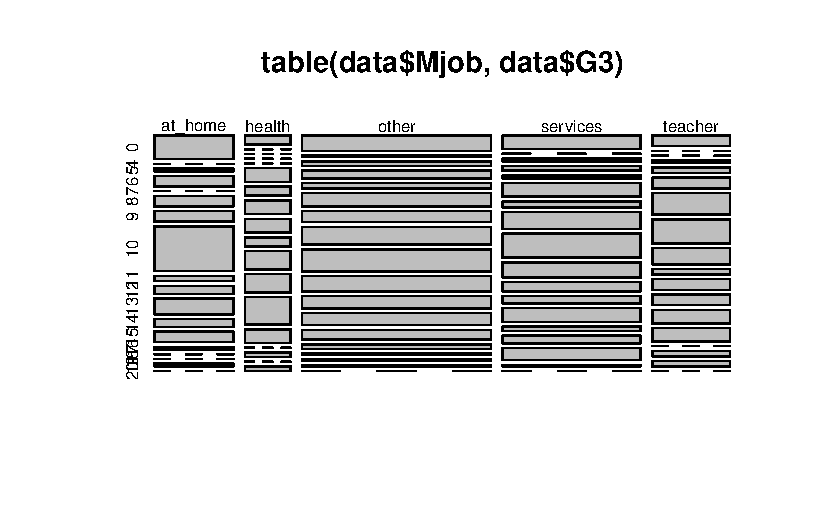
\includegraphics{education_files/figure-pdf/unnamed-chunk-3-1.pdf}

\begin{Shaded}
\begin{Highlighting}[]
\FunctionTok{lm}\NormalTok{(data}\SpecialCharTok{$}\NormalTok{G3 }\SpecialCharTok{\textasciitilde{}}\NormalTok{ data}\SpecialCharTok{$}\NormalTok{Medu)}
\end{Highlighting}
\end{Shaded}

\begin{verbatim}

Call:
lm(formula = data$G3 ~ data$Medu)

Coefficients:
(Intercept)    data$Medu  
     7.9167       0.9088  
\end{verbatim}




\end{document}
